\chapter{Theoretical Framework}
\label{ch:theory}

\blindtext

\section{Fundamentals}
\label{sec:fundamentals}

\blindtext
%
\begin{equation}
x = \frac{-b \pm \sqrt{b^2 - 4ac}}{2a}
\end{equation}
% COMMENT: An empty line creates a new paragraph (inducing indentation). 
% To keep the code readable without starting a new paragraph after 
% an equation, use a single "%" line.
\blindtext
%
\begin{equation}\label{eq:emc2}
E=mc^2
\end{equation}
%
\Cref{eq:emc2} shows the equivalence of energy $E$ and mass $m$.

\begin{figure}[!b]
	\centering
	\begin{subfigure}{0.4\textwidth}
		\centering
		\includegraphics[width=\linewidth]{example-image-a}
		\caption{Variant A}
		\label{fig:a}
	\end{subfigure}
	%\par\medskip
	\begin{subfigure}{0.4\textwidth}
		\centering
		\includegraphics[width=\linewidth]{example-image-b}
		\caption{Variant B}
		\label{fig:b}
	\end{subfigure}
	\caption{Comparison of two schematic model variants.}
	\label{fig:comparison}
\end{figure}
%
\blindtext
%
%\begin{figure}
%	\centering
%	\resizebox{0.3\textwidth}{!}{%
%		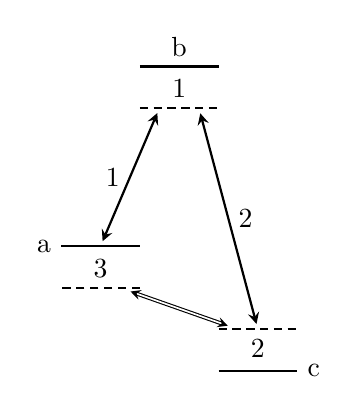
\begin{tikzpicture}[
	scale=0.5,
	level/.style={thick},
	virtual/.style={thick,densely dashed},
	trans/.style={thick,<->,shorten >=2pt,shorten <=2pt,>=stealth},
	classical/.style={thin,double,<->,shorten >=4pt,shorten <=4pt,>=stealth}
	]
	% Draw the energy levels.
	\draw[level] (2cm,-2em) -- (0cm,-2em) node[left] {\ket{a}};
	\draw[level] (2cm,11em) -- (4cm,11em) node[midway,above] {\ket{b}};
	\draw[level] (4cm,-11em) -- (6cm,-11em) node[right] {\ket{c}};
	% Draw the virtual levels.
	\draw[virtual] (2cm,8em) -- (4cm,8em) node[midway,above] {\De{1}};
	\draw[virtual] (4cm,-8em) -- (6cm,-8em) node[midway,below] {\De{2}};
	\draw[virtual] (2cm,-5em) -- (0cm,-5em) node[midway,above] {\De{3}};
	% Draw the transitions.
	\draw[trans] (1cm,-2em) -- (2.5cm,8em) node[midway,left] {\Om{1}};
	\draw[trans] (3.5cm,8em) -- (5cm,-8em) node[midway,right] {\Om{2}};
	\draw[classical] (4.5cm,-8em) -- (1.5cm,-5em) node[midway,below] {\Ga{}};
\end{tikzpicture}
%	}
%	\caption[
%	A simple level diagram with some transitions
%	]{
%		A simple level diagram with some transitions. Taken from:
%	}
%\end{figure}
%
\blindtext
%
\begin{align}
  (x + 3)^2 - 5 &= x^2 + 6x + 9 - 5 \\
&= x^2 + 6x + 4
\end{align}
%
\blindtext[3]
%
\begin{align*}
	\int_a^bf(x)\mathrm{d}x &= \int_a^b\left(\sum_{k=0}^\infty a_kx^k\right)\Big(\lim_{\varepsilon\to0}e^{\varepsilon x}\Big)\mathrm{d}x \\
	&= \lim_{\varepsilon\to0}\sum_{k=0}^\infty\int_a^ba_kx^ke^{\varepsilon x}\mathrm{d}x \\
	&= \lim_{\varepsilon\to0}\sum_{k=0}^\infty a_k\int_a^b\left(\frac{\mathrm{d}^k}{\mathrm{d}\varepsilon^k}e^{\varepsilon x}\right)\mathrm{d}x \\
	&= \lim_{\varepsilon\to0}\left(\sum_{k=0}^\infty a_k\frac{\mathrm{d}^k}{\mathrm{d}\varepsilon^k}\right) \left(\int_a^be^{\varepsilon x}\mathrm{d}x\right) \\
	&= \lim_{\varepsilon\to0} f\left(\frac{\mathrm{d}}{\mathrm{d}\varepsilon}\right)\frac{e^{\varepsilon b}-e^{\varepsilon a}}{\varepsilon}.
\end{align*}
%
%\blindtext

\section{Models and Assumptions}
\label{sec:models-assumptiopns}

\blindtext
%
\begin{figure}
	\centering
	\resizebox{0.3\textwidth}{!}{%
		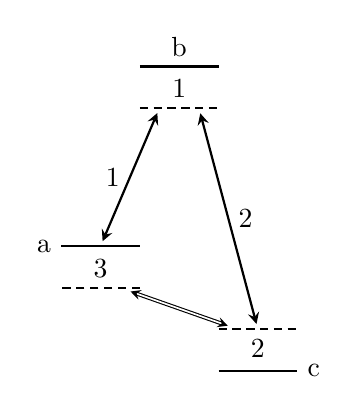
\begin{tikzpicture}[
	scale=0.5,
	level/.style={thick},
	virtual/.style={thick,densely dashed},
	trans/.style={thick,<->,shorten >=2pt,shorten <=2pt,>=stealth},
	classical/.style={thin,double,<->,shorten >=4pt,shorten <=4pt,>=stealth}
	]
	% Draw the energy levels.
	\draw[level] (2cm,-2em) -- (0cm,-2em) node[left] {\ket{a}};
	\draw[level] (2cm,11em) -- (4cm,11em) node[midway,above] {\ket{b}};
	\draw[level] (4cm,-11em) -- (6cm,-11em) node[right] {\ket{c}};
	% Draw the virtual levels.
	\draw[virtual] (2cm,8em) -- (4cm,8em) node[midway,above] {\De{1}};
	\draw[virtual] (4cm,-8em) -- (6cm,-8em) node[midway,below] {\De{2}};
	\draw[virtual] (2cm,-5em) -- (0cm,-5em) node[midway,above] {\De{3}};
	% Draw the transitions.
	\draw[trans] (1cm,-2em) -- (2.5cm,8em) node[midway,left] {\Om{1}};
	\draw[trans] (3.5cm,8em) -- (5cm,-8em) node[midway,right] {\Om{2}};
	\draw[classical] (4.5cm,-8em) -- (1.5cm,-5em) node[midway,below] {\Ga{}};
\end{tikzpicture}
	}
	\caption[
	A simple level diagram with some transitions
	]{
		A simple level diagram with some transitions. Taken from:
	}
\end{figure}
%
\blindtext

\blindtext
%
\begin{figure}
	\centering
	\resizebox{\textwidth}{!}{%
	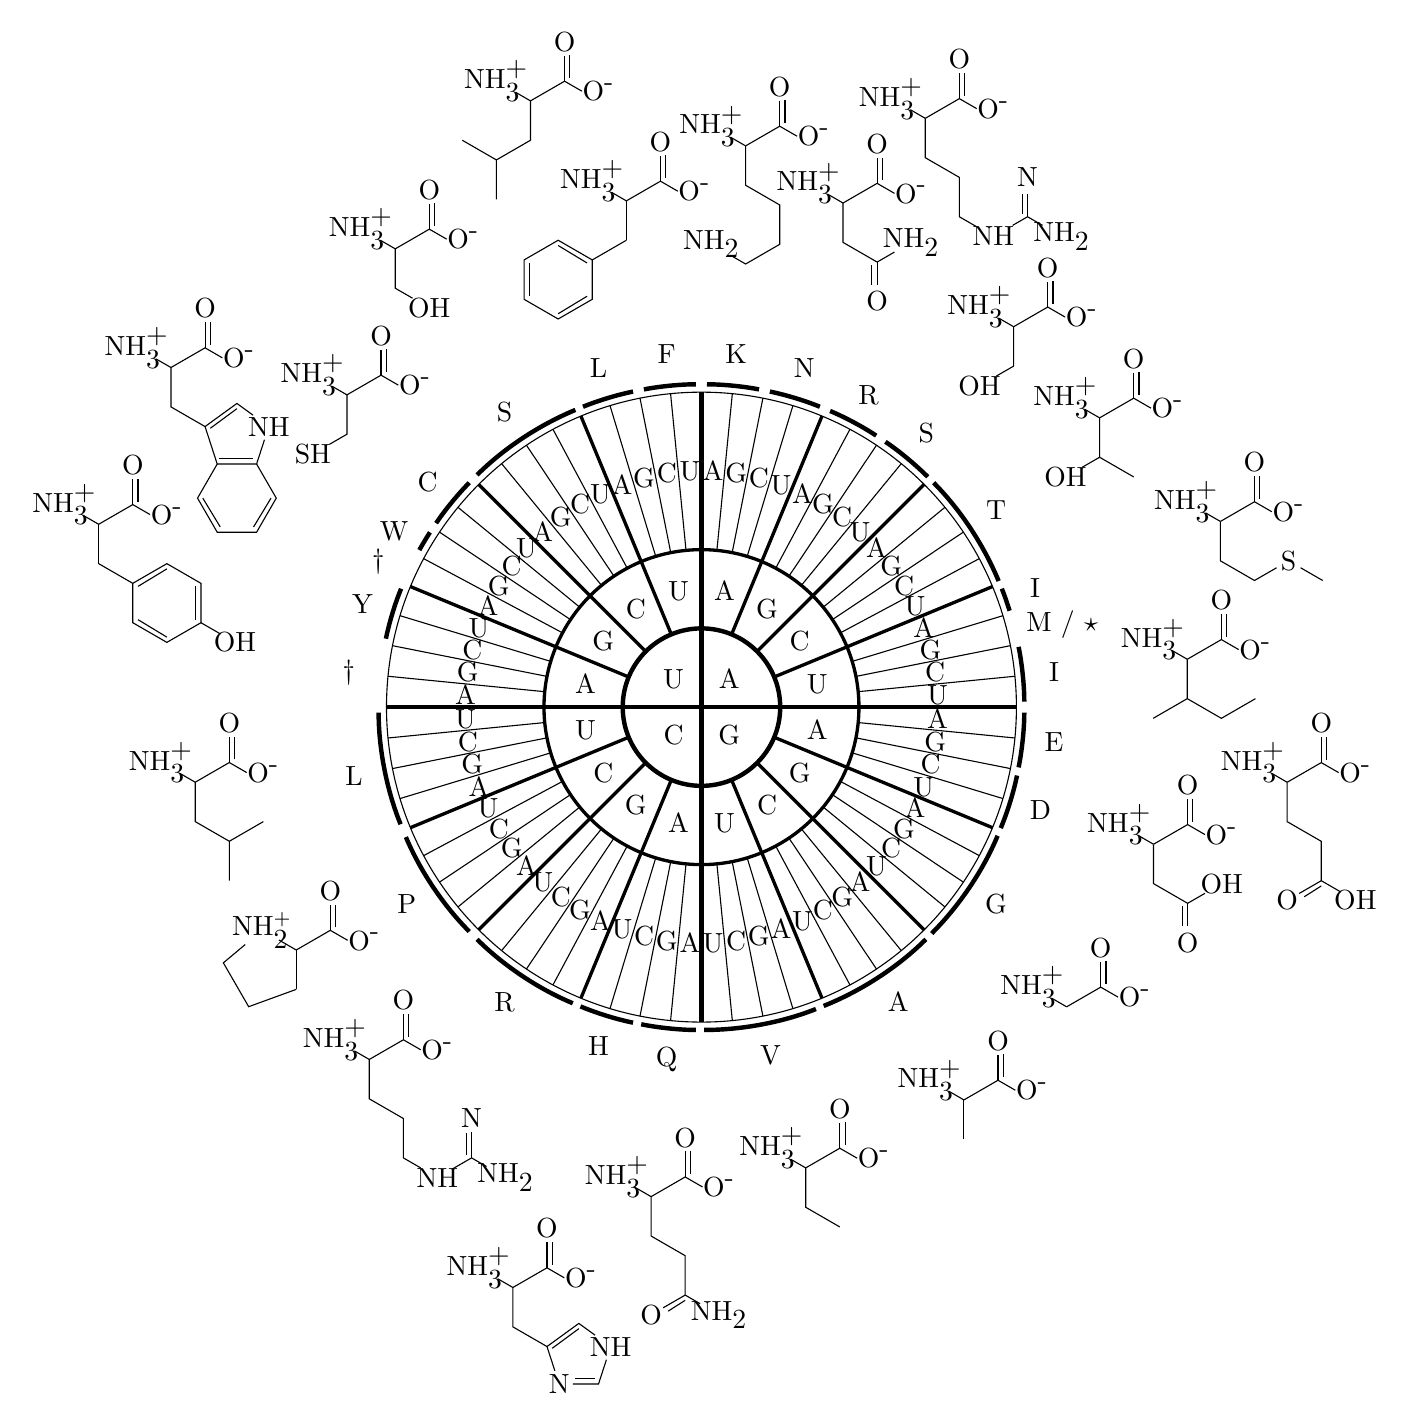
\begin{tikzpicture}
	\tikzstyle{every node}=[inner sep=1.7pt,anchor=center]
	%	to_x and from_x styles denote bonds terminating or starting in labeled nodes. x denotes the number of letters in the node label.
	\tikzstyle{to_1}=[shorten >=5pt]
	\tikzstyle{to_1i}=[shorten >=6pt]
	\tikzstyle{to_2}=[shorten >=7pt]
	\tikzstyle{to_3}=[shorten >=8pt]
	\tikzstyle{from_1}=[shorten <=5pt]
	\tikzstyle{from_1i}=[shorten <=6pt]
	\tikzstyle{from_2}=[shorten <=8pt]
	\begin{scope}
		\draw [ultra thick] circle(1cm);
		\draw [ultra thick] (0:4)--(180:4) (90:4)--(270:4);
		\foreach \a/\l in {45/A,135/G,225/C,315/U}{
			\node at (90-\a:0.5cm) {\l};
		}
		\draw [very thick] circle(2cm);
		\foreach \A in {90,0,270,180}{
			\foreach \a/\l in {22.5/A,45/G,67.5/C,90/U}{
				\draw [very thick] (\A+\a:1) -- (\A+\a:4);
				\node at (\A-\a+11.25:1.5) {\l};
			}
		}
		\draw circle(4cm) (0:4)--(180:4) (90:4)--(270:4);
		\foreach \A in {90,180,270,0}{
			\foreach \a in {0,22.5,45,67.5}{
				\foreach \i/\l in {5.625/A,11.25/G,16.875/C,22.5/U}{
					\draw (\A+\a+\i:2) -- (\A+\a+\i:4);
					\node at (\A-\a-\i+2.8125:3) {\l};
				}
			}
		}
	\end{scope}
	\begin{scope}[scale=0.5]	% Lysine
		\draw[ultra thick,shorten >=2pt,shorten <=2pt] (90:8.2)
		arc(90:90-2*5.625:8.2);
		\path (90-0.8*5.625:14.3) node (zero) {};
		\draw[to_2]  (zero.center)	-- ++(30:1) node (CO) {}  
		-- +(330:1) node [anchor=base] {O$^{\mbox{-}}$};
		\draw[to_1]  (CO.center) 	-- +(90:1) node (Od) {O};
		\draw[to_1i] (CO.30)		-- +(90:1);
		\draw[to_3]  (zero.center)	-- ++(150:1) node {NH$_{\mbox{3}}^{\mbox{+}}$};
		\draw[to_3]  (zero.center)	-- ++(270:1) node(Cb){}
		-- ++(330:1) node (Cc) {}
		-- ++(270:1) node (Cd) {}
		-- ++(210:1) node (Ce) {}
		-- ++(150:1) node (Cf) {NH$_{\mbox{2}}$};
	\end{scope}
	\begin{scope}[scale=0.5]	% Asparagine
		\draw[ultra thick,shorten >=2pt,shorten <=2pt] (90-2*5.625:8.2)
		arc(90-2*5.625:90-4*5.625:8.2);
		\path (90-3.5*3.625-3:13.3) node (zero) {};
		\draw[to_2]  (zero.center)	-- ++(30:1) node (CO) {} 
		-- +(330:1) node [anchor=base] {O$^{\mbox{-}}$};
		\draw[to_1]  (CO.center)	-- +(90:1) node (Od) {O};
		\draw[to_1i] (CO.30)		-- +(90:1);
		\draw[to_3]  (zero.center)	-- ++(150:1) node {NH$_{\mbox{3}}^{\mbox{+}}$};
		\draw[to_2]  (zero.center)	-- ++(270:1) node(Cb){}
		-- ++(330:1) node (Cc) {}
		-- +(30:1) node (Cd) {NH$_{\mbox{2}}$};
		\draw[to_1i] (Cc.center)	-- +(270:1) node (O) {};
		\draw[to_1]  (Cc.210)		-- (O.150);
		\path (O.center) node {O};
	\end{scope}
	\begin{scope}[scale=0.5]	% Arginine
		\draw[ultra thick,shorten >=2pt,shorten <=2pt] (90-22.5:8.2)
		arc(90-22.5:90-33.75:8.2);
		\path (90-3.7*5.625:16) node (zero) {};
		\draw[to_2]  (zero.center)	-- ++(30:1) node (CO) {}
		-- +(330:1) node [anchor=base] {O$^{\mbox{-}}$};
		\draw[to_1]  (CO.center)	-- +(90:1) node (Od) {O};
		\draw[to_1i] (CO.30)		-- +(90:1);
		\draw[to_3]  (zero.center)	-- ++(150:1) node {NH$_{\mbox{3}}^{\mbox{+}}$};
		\draw[to_2]  (zero.center)	-- ++(270:1) node(Cb){}
		-- ++(330:1) node (Cc) {}
		-- ++(270:1) node (Cd) {}
		-- ++(330:1) node (NH1) {NH};
		\draw[from_2,to_3]  (NH1.center)	-- ++(30:1) node (Ce) {}
		-- ++(330:1) node {NH$_{\mbox{2}}$};
		\draw[to_1i] (Ce.center)	-- ++(90:1) node (N2) {};
		\draw[to_1]  (Ce.150)		-- (N2.210);
		\path (N2) node {N};
	\end{scope}
	\begin{scope}[scale=0.5]	% Serine
		\draw[ultra thick,shorten >=1pt,shorten <=2pt] (90-22.5-2*5.625:8.2)
		arc(90-33.75:90-33.75-11.25:8.2);
		\path (90-7*5.625:12.5) node (zero) {};
		\draw[to_2]  (zero.center)	-- ++(30:1) node (CO) {}
		-- +(330:1) node [anchor=base] {O$^{\mbox{-}}$};
		\draw[to_1]  (CO.center)	-- +(90:1) node (Od) {O};
		\draw[to_1i] (CO.30)		-- +(90:1);
		\draw[to_3]  (zero.center)	-- ++(150:1) node {NH$_{\mbox{3}}^{\mbox{+}}$};
		\draw[to_2]  (zero.center)	-- ++(270:1) node(Cb){} -- ++(210:1) node (Cc) {OH};
	\end{scope}
	\begin{scope}[scale=0.5]	% Threonine
		\draw[ultra thick,shorten >=1pt,shorten <=2pt] (90-45:8.2)
		arc(90-45:90-67.5:8.2);
		\path (90-45-0.8*11.25:12.5) node (zero) {};
		\draw[to_2]  (zero.center)	-- ++(30:1) node (CO) {}
		-- +(330:1) node [anchor=base] {O$^{\mbox{-}}$};
		\draw[to_1]  (CO.center)	-- +(90:1) node (Od) {O};
		\draw[to_1i] (CO.30)		-- +(90:1);
		\draw[to_3]  (zero.center)	-- ++(150:1) node {NH$_{\mbox{3}}^{\mbox{+}}$};
		\draw[to_2]  (zero.center)	-- ++(270:1) node(Cb){}
		-- ++(330:1) node (Cc) {} (Cb.center)
		-- +(210:1) node {OH};
	\end{scope}
	\begin{scope}[scale=0.5]	% Methionine
		\draw[ultra thick,shorten >=1pt,shorten <=2pt] (90-67.5:8.2)
		arc(90-67.5:90-67.5-5.625:8.2);
		\path (90-67.5-0.5*5.625:14) node (zero) {};
		\draw[to_2]  (zero.center)	-- ++(30:1) node (CO) {}
		-- +(330:1) node [anchor=base] {O$^{\mbox{-}}$};
		\draw[to_1]  (CO.center)	-- +(90:1) node (Od) {O};
		\draw[to_1i] (CO.30)		-- +(90:1);
		\draw[to_3]  (zero.center)	-- ++(150:1) node {NH$_{\mbox{3}}^{\mbox{+}}$};
		\draw[to_1]  (zero.center)	-- ++(270:1) node(Cb){}
		-- ++(330:1) node (Cc) {}
		-- ++(30:1) node (Cd) {S};
		\draw[from_1] (Cd.center)	-- +(330:1);
	\end{scope}
	\begin{scope}[scale=0.5]	% Isoleucine
		\draw[ultra thick,shorten >=1pt,shorten <=2pt] (0:8.2)
		arc(0:11.25:8.2);
		\path (1.0*5.625:12.4) node (zero) {};
		\draw[to_2]  (zero.center)	-- ++(30:1) node (CO) {}
		-- +(330:1) node [anchor=base] {O$^{\mbox{-}}$};
		\draw[to_1]  (CO.center)	-- +(90:1) node (Od) {O};
		\draw[to_1i] (CO.30)		-- +(90:1);
		\draw[to_3]  (zero.center)	-- ++(150:1) node {NH$_{\mbox{3}}^{\mbox{+}}$};
		\draw	     (zero.center)	-- ++(270:1) node(Cb){}
		-- ++(330:1) node (Cc) {}
		-- +(30:1) node (Cd) {} (Cb.center)
		-- +(210:1) node (Ce) {};
	\end{scope}
	\begin{scope}[scale=0.5]	% Glutamic acid
		\draw[ultra thick,shorten >=1pt,shorten <=2pt] (0:8.2)
		arc(0:-11.25:8.2);
		\path (-1.3*5.625:15) node (zero) {};
		\draw[to_2]  (zero.center)	-- ++(30:1) node (CO) {}
		-- +(330:1) node [anchor=base] {O$^{\mbox{-}}$};
		\draw[to_1]  (CO.center)  	-- +(90:1) node (Od) {O};
		\draw[to_1i] (CO.30)  		-- +(90:1);
		\draw[to_3]  (zero.center) 	-- ++(150:1) node {NH$_{\mbox{3}}^{\mbox{+}}$};
		\draw[to_1i] (zero.center) 	-- ++(270:1) node(Cb){} 
		-- ++(330:1) node (Cc) {} 
		-- ++(270:1) node (Cd) {}
		-- ++(330:1) node (NH) {OH};
		\draw[to_1]  (Cd.center) 	-- +(210:1) node (O) {};
		\draw[to_1i] (Cd.270) 		-- (O.300);
		\path (O.center) node {O};
	\end{scope}
	\begin{scope}[scale=0.5]	% Aspartic acid
		\draw[ultra thick,shorten >=1pt,shorten <=2pt] (-11.25:8.2)
		arc(-11.25:-22.5:8.2);
		\path (-11.25-5.625:12) node (zero) {};
		\draw[to_2]  (zero.center)	-- ++(30:1) node (CO) {}
		-- +(330:1) node [anchor=base] {O$^{\mbox{-}}$};
		\draw[to_1]  (CO.center) 	-- +(90:1) node (Od) {O};
		\draw[to_1i] (CO.30)		-- +(90:1);
		\draw[to_3]  (zero.center)	-- ++(150:1) node {NH$_{\mbox{3}}^{\mbox{+}}$};
		\draw[to_2]  (zero.center)	-- ++(270:1) node(Cb){}
		-- ++(330:1) node (Cc) {}
		-- +(30:1) node (Cd) {OH};
		\draw[to_1i] (Cc.center)	-- +(270:1) node (O) {};
		\draw[to_1]  (Cc.210)		-- (O.150);
		\path (O.center) node {O};
	\end{scope}
	\begin{scope}[scale=0.5]	% Glycine
		\draw[ultra thick,shorten >=1pt,shorten <=2pt] (-22.5:8.2)
		arc(-22.5:-45:8.2);
		\path (-33.75-1*5.625:12) node (zero) {};
		\draw[to_2]  (zero.center)	-- ++(30:1) node (CO) {}
		-- +(330:1) node [anchor=base] {O$^{\mbox{-}}$};
		\draw[to_1]  (CO.center)	-- +(90:1) node (Od) {O};
		\draw[to_1i] (CO.30)		-- +(90:1);
		\draw[to_3]  (zero.center)	-- ++(150:1) node {NH$_{\mbox{3}}^{\mbox{+}}$};
	\end{scope}
	\begin{scope}[scale=0.5]	% Alanine
		\draw[ultra thick,shorten >=1pt,shorten <=2pt] (-45:8.2)
		arc(-45:-68.25:8.2);
		\path (-45-11.25:12) node (zero) {};
		\draw[to_2]  (zero.center)	-- ++(30:1) node (CO) {}
		-- +(330:1) node [anchor=base] {O$^{\mbox{-}}$};
		\draw[to_1]  (CO.center)	-- +(90:1) node (Od) {O};
		\draw[to_1i] (CO.30)		-- +(90:1);
		\draw[to_3]  (zero.center)	-- ++(150:1) node {NH$_{\mbox{3}}^{\mbox{+}}$};
		\draw	     (zero.center)	-- ++(270:1) node(Cb){};
	\end{scope}
	\begin{scope}[scale=0.5]	% Valine
		\draw[ultra thick,shorten >=1pt,shorten <=2pt] (-68.25:8.2)
		arc(-68.25:-90:8.2);
		\path (-68.25-0.8*11.25:12) node (zero) {};
		\draw[to_2]  (zero.center)	-- ++(30:1) node (CO) {}
		-- +(330:1) node [anchor=base] {O$^{\mbox{-}}$};
		\draw[to_1]  (CO.center)	-- +(90:1) node (Od) {O};
		\draw[to_1i] (CO.30)		-- +(90:1);
		\draw[to_3]  (zero.center)	-- ++(150:1) node {NH$_{\mbox{3}}^{\mbox{+}}$};
		\draw (zero.center)		-- ++(270:1) node(Cb){}
		-- ++(330:1) node (Cc) {};
	\end{scope}
	\begin{scope}[scale=0.5]	% Glutamine
		\draw[ultra thick,shorten >=1pt,shorten <=2pt] (-90:8.2)
		arc(-90:-101.25:8.2);
		\path (-90.25-5.625:12.5) node (zero) {};
		\draw[to_2]  (zero.center)	-- ++(30:1) node (CO) {}
		-- +(330:1) node [anchor=base] {O$^{\mbox{-}}$};
		\draw[to_1]  (CO.center)	-- +(90:1) node (Od) {O};
		\draw[to_1i] (CO.30)		-- +(90:1);
		\draw[to_2]  (zero.center)	-- ++(150:1) node {NH$_{\mbox{3}}^{\mbox{+}}$};
		\draw[to_3]  (zero.center)	-- ++(270:1) node(Cb){}
		-- ++(330:1) node (Cc) {}
		-- ++(270:1) node (Cd) {}
		-- ++(330:1) node (NH) {NH$_{\mbox{2}}$};
		\draw[to_1]  (Cd.center)	-- +(210:1) node (O) {};
		\draw[to_1i] (Cd.270)		-- (O.300);
		\path (O.center) node {O};
	\end{scope}
	\begin{scope}[scale=0.5]	% Histidine
		\draw[ultra thick,shorten >=1pt,shorten <=2pt] (-101.25:8.2)
		arc(-101.25:-101.25-11.25:8.2);
		\path (-101.25-1.2*5.625:15.5) node (zero) {};
		\draw[to_2]  (zero.center)	-- ++(30:1) node (CO) {}
		-- +(330:1) node [anchor=base] {O$^{\mbox{-}}$};
		\draw[to_1]  (CO.center)	-- +(90:1) node (Od) {O};
		\draw[to_1i] (CO.30)		-- +(90:1);
		\draw[to_3]  (zero.center)	-- ++(150:1) node {NH$_{\mbox{3}}^{\mbox{+}}$};
		\draw        (zero.center)	-- ++(270:1) node(Cb){}
		-- ++(330:1) node(Cc){};
		\draw[to_2]  (Cc.center)	-- ++(108-1*72:1) node (Cd) {}
		-- ++(108-2*72:1) node (Ce) {NH};
		\draw[from_1,to_1] (Ce.center)	-- ++(108-3*72:1) node (Cf) {}
		-- ++(108-4*72:1) node (Cg) {};
		\draw[from_1] (Cg.center)	-- (Cc.center);
		\draw         (Cc.198+2*72)	-- (Cd.198+1*72);
		\draw[from_1] (Cg.72)		-- (Cf.198+4*72);
		\draw (Cg.center) node {N};
	\end{scope}
	\begin{scope}[scale=0.5]	% Arginine
		\draw[ultra thick,shorten >=2pt,shorten <=2pt] (-90-22.5:8.2)
		arc(-90-22.5:-90-45:8.2);
		\path (-90-7.7*5.625:12.3) node (zero) {};
		\draw[to_2]  (zero.center)	-- ++(30:1) node (CO) {}
		-- +(330:1) node [anchor=base] {O$^{\mbox{-}}$};
		\draw[to_1]  (CO.center)	-- +(90:1) node (Od) {O};
		\draw[to_1i] (CO.30)		-- +(90:1);
		\draw[to_3]  (zero.center)	-- ++(150:1) node {NH$_{\mbox{3}}^{\mbox{+}}$};
		\draw[to_2]  (zero.center)	-- ++(270:1) node(Cb){}
		-- ++(330:1) node (Cc) {}
		-- ++(270:1) node (Cd) {}
		-- ++(330:1) node (NH1) {NH};
		\draw[from_1i,to_3] (NH1.center)-- ++(30:1) node (Ce) {}
		-- ++(330:1) node {NH$_{\mbox{2}}$};
		\draw[to_1]  (Ce.center)	-- ++(90:1) node (N2) {};
		\draw[shorten >=4pt] (Ce.150)	-- (N2.210);
		\path (N2) node {N};
	\end{scope}
	\begin{scope}[scale=0.5]	% Proline
		\draw[ultra thick,shorten >=2pt,shorten <=2pt] (-90-45:8.2)
		arc(-90-45:-90-45-22.25:8.2);
		\path (-90-10.5*5.625:12) node (zero) {};
		\draw[to_2]  (zero.center)	-- ++(30:1) node (CO) {}
		-- +(330:1) node [anchor=base] {O$^{\mbox{-}}$};
		\draw[to_1]  (CO.center)	-- +(90:1) node (Od) {O};
		\draw[to_1i] (CO.30)		-- +(90:1);
		\draw[to_2]  (zero.center)	-- ++(150:1) node (nh) {NH$_{\mbox{2}}^+$};
		\draw        (zero.center)	-- ++(270:1) node(Cb){};
		\path        (Cb.center)	-- +(150:1) node (x) {};
		\path        (x.center)  	+(170:1) node (Cd) {};
		\path        (x.center)  	+(250:1) node (Cc) {};
		\draw[to_3]  (Cb.center)	-- (Cc.center)
		-- (Cd.center)
		-- (nh.center);
	\end{scope}
	\begin{scope}[scale=0.5]	% Leucine
		\draw[ultra thick,shorten >=2pt,shorten <=2pt] (180:8.2)
		arc(180:180+22.25:8.2);
		\path (-90-14.5*5.625:13) node (zero) {};
		\draw[to_2]  (zero.center)	-- ++(30:1) node (CO) {}
		-- +(330:1) node [anchor=base] {O$^{\mbox{-}}$};
		\draw[to_1]  (CO.center)	-- +(90:1) node (Od) {O};
		\draw[to_1i] (CO.30)		-- +(90:1);
		\draw[to_3]  (zero.center)	-- ++(150:1) node {NH$_{\mbox{3}}^{\mbox{+}}$};
		\draw (zero.center)		-- ++(270:1) node(Cb){}
		-- ++(330:1) node (Cc) {}
		-- +(30:1) node (Cd) {} (Cc.center)
		-- +(270:1) node (Ce) {};
	\end{scope}
	\begin{scope}[scale=0.5]	% Tyrosine
		\draw[ultra thick,shorten >=2pt,shorten <=2pt] (180-11.25:8.2)
		arc(180-11.25:180-22.5:8.2);
		\path (180-3*5.625:16) node (zero) {};
		\draw[to_2]  (zero.center)	-- ++(30:1) node (CO) {}
		-- +(330:1) node [anchor=base] {O$^{\mbox{-}}$};
		\draw[to_1]  (CO.center)	-- +(90:1) node (Od) {O};
		\draw[to_1i] (CO.30)		-- +(90:1);
		\draw[to_3]  (zero.center)	-- ++(150:1) node {NH$_{\mbox{3}}^{\mbox{+}}$};
		\draw 	     (zero.center)	-- ++(270:1) node(Cb){};
		\draw	     (Cb.center)	-- ++(330:1) node (Cc) {}
		-- ++(30:1) node (Cd) {}
		-- ++(330:1) node (Ce) {}
		-- ++(270:1) node (Cf) {}
		-- ++(210:1) node (Cg) {}
		-- ++(150:1) node (Ch) {}
		-- ++(90:1);
		\draw        (Cc.330)		-- (Cd.270);
		\draw        (Ce.210)		-- (Cf.150);
		\draw        (Cg.90)		-- (Ch.30);
		\draw[to_1i] (Cf.center)	-- +(330:1) node (OH) {OH};
	\end{scope}
	\begin{scope}[scale=0.5]	% Tryptophane
		\draw[ultra thick,shorten >=2pt,shorten <=2pt] (180-22.5-5.625:8.2)
		arc(180-22.5-5.625:180-22.5-11.25:8.2);
		\path (180-22.5-1.8*5.625:16) node (zero) {};
		\draw[to_2]  (zero.center)	-- ++(30:1) node (CO) {}
		-- +(330:1) node [anchor=base] {O$^{\mbox{-}}$};
		\draw[to_1]  (CO.center)	-- +(90:1) node (Od) {O};
		\draw[to_1i] (CO.30)		-- +(90:1);
		\draw[to_3]  (zero.center)	-- ++(150:1) node {NH$_{\mbox{3}}^{\mbox{+}}$};
		\draw 	     (zero.center)	-- ++(270:1) node(Cb){}
		-- ++(330:1) node(Cc){};
		\draw[to_2]  (Cc.center)	-- ++(108-1*72:1) node (Cd) {}
		-- ++(108-2*72:1) node (Ce) {NH};
		\draw[from_1](Ce.center)	-- ++(108-3*72:1) node (Cf) {}
		-- ++(108-4*72:1) node (Cg) {};
		\draw 	     (Cg.center)	-- (Cc.center);
		\draw        (Cc.198+2*72)	-- (Cd.198+1*72);
		\draw 	     (Cg.72)		-- (Cf.198+4*72);
		\draw	     (Cg.center)	-- ++(240:1) node (Ch) {}
		-- ++(300:1) node (Ci) {}
		-- ++(0:1) node (Cj) {}
		-- ++(60:1) node (Ck) {}
		-- ++(120:1) node (Cl) {};
		\draw	     (Ch.0)		-- (Ci.60);
		\draw	     (Cj.120)		-- (Ck.180);
	\end{scope}
	\begin{scope}[scale=0.5]	% Cysteine
		\draw[ultra thick,shorten >=2pt,shorten <=2pt] (180-45+11.25:8.2)
		arc(180-45+11.25:180-45:8.2);
		\path (180-45+11.25-1*7.625:12) node (zero) {};
		\draw[to_2]  (zero.center)	-- ++(30:1) node (CO) {}
		-- +(330:1) node [anchor=base] {O$^{\mbox{-}}$};
		\draw[to_1]  (CO.center)	-- +(90:1) node (Od) {O};
		\draw[to_1i] (CO.30)		-- +(90:1);
		\draw[to_3]  (zero.center)	-- ++(150:1) node {NH$_{\mbox{3}}^{\mbox{+}}$};
		\draw[to_2]  (zero.center)	-- ++(270:1) node(Cb){}
		-- ++(210:1) node (Cc) {SH};
	\end{scope}
	\begin{scope}[scale=0.5]	% Serine
		\draw[ultra thick,shorten >=1pt,shorten <=2pt] (90+45:8.2)
		arc(90+45:90+45-22.5:8.2);
		\path (90+45-11.25+0*5.625:14) node (zero) {};
		\draw[to_2]  (zero.center)	-- ++(30:1) node (CO) {}
		-- +(330:1) node [anchor=base] {O$^{\mbox{-}}$};
		\draw[to_1]  (CO.center)	-- +(90:1) node (Od) {O};
		\draw[to_1i] (CO.30)		-- +(90:1);
		\draw[to_3]  (zero.center)	-- ++(150:1) node {NH$_{\mbox{3}}^{\mbox{+}}$};
		\draw[to_2]  (zero.center)	-- ++(270:1) node(Cb){}
		-- ++(330:1) node (Cc) {OH};
	\end{scope}
	\begin{scope}[scale=0.5]	% Leucine
		\draw[ultra thick,shorten >=2pt,shorten <=2pt] (90+22.5:8.2)
		arc(90+22.5:90+11.25:8.2);
		\path (90+22.5-1.2*5.625:16) node (zero) {};
		\draw[to_2]  (zero.center)	-- ++(30:1) node (CO) {}
		-- +(330:1) node [anchor=base] {O$^{\mbox{-}}$};
		\draw[to_1]  (CO.center)	-- +(90:1) node (Od) {O};
		\draw[to_1i] (CO.30)		-- +(90:1);
		\draw[to_3]  (zero.center)	-- ++(150:1) node {NH$_{\mbox{3}}^{\mbox{+}}$};
		\draw 	     (zero.center)	-- ++(270:1) node(Cb){}
		-- ++(210:1) node (Cc) {}
		-- +(150:1) node (Cd) {} (Cc.center)
		-- +(270:1) node (Ce) {};
	\end{scope}
	\begin{scope}[scale=0.5]	% Phenylalanine
		\draw[ultra thick,shorten >=2pt,shorten <=2pt] (90+11.25:8.2)
		arc(90+11.25:90:8.2);
		\path (90+1.5*5.625:13) node (zero) {};
		\draw[to_2]  (zero.center)	-- ++(30:1) node (CO) {}
		-- +(330:1) node [anchor=base] {O$^{\mbox{-}}$};
		\draw[to_1]  (CO.center)	-- +(90:1) node (Od) {O};
		\draw[to_1i] (CO.30)		-- +(90:1);
		\draw[to_3]  (zero.center)	-- ++(150:1) node {NH$_{\mbox{3}}^{\mbox{+}}$};
		\draw	     (zero.center)	-- ++(270:1) node(Cb){};
		\draw	     (Cb.center)	-- ++(210:1) node (Cc) {}
		-- ++(150:1) node (Cd) {}
		-- ++(210:1) node (Ce) {}
		-- ++(270:1) node (Cf) {}
		-- ++(330:1) node (Cg) {}
		-- ++(30:1) node (Ch) {}
		-- ++(90:1);
		\draw	     (Cc.210)		-- (Cd.270);
		\draw	     (Ce.330)		-- (Cf.30);
		\draw	     (Cg.90)		-- (Ch.150);
	\end{scope}
	\node at (90-1*5.625:4.5) {K};
	\node at (90-3*5.625:4.5) {N};
	\node at (90-5*5.625:4.5) {R};
	\node at (90-7*5.625:4.5) {S};
	\node at (90-10*5.625:4.5) {T};
	\node at (90-12.5*5.625:4.5) {I};
	\node at (90-13.7*5.625:4.7) {M / $\star$};
	\node at (90-15*5.625:4.5) {I};
	\node at (90-17*5.625:4.5) {E};
	\node at (90-19*5.625:4.5) {D};
	\node at (90-22*5.625:4.5) {G};
	\node at (90-26*5.625:4.5) {A};
	\node at (90-30*5.625:4.5) {V};
	\node at (90-33*5.625:4.5) {Q};
	\node at (90-35*5.625:4.5) {H};
	\node at (90-38*5.625:4.5) {R};
	\node at (90-42*5.625:4.5) {P};
	\node at (90-46*5.625:4.5) {L};
	\node at (90-49*5.625:4.5) {$\dagger$};
	\node at (90-51*5.625:4.5) {Y};
	\node at (90-52.3*5.625:4.5) {$\dagger$};
	\node at (90-53.3*5.625:4.5) {W};
	\node at (90-55*5.625:4.5) {C};
	\node at (90-58*5.625:4.5) {S};
	\node at (90-61*5.625:4.5) {L};
	\node at (90-63*5.625:4.5) {F};
\end{tikzpicture}
	}
	\caption[
		A table of the RNA codons together with the amino acids they encode
	]{
		A table of the RNA codons together with the amino acids they encode. Taken from:
	}
\end{figure}